\section{Открытый корпус вепсского и карельского языков (ВепКар)} \label{sect_VepKar_about}

В этом подразделе дадим краткую справку о том, что из себя представляет 
лингвистический корпус ВепКар, в основе которого лежит 
разрабатываемый комплекс компьютерных программ.

В соответствии с классификацией, предложенной 
в учебнике по корпусной лингвистике~\cite[с.~12]{Zakharov2005}, 
разрабатываемый \emph{Открытый корпус вепсского и карельского языков}: 
\renewcommand{\outlinei}{itemize}
\renewcommand{\outlineii}{itemize}
\begin{outline}
    \1 является многоязычным корпусом;
    \1 является полнотекстовым корпусом;
    \1 предоставляет пользователям доступ к полным текстам документов в отличие, 
    например, от НКРЯ\footnote{Национальный 
    корпус русского языка (НКРЯ) содержит 
        полные тексты произведений~\cite[с.~12]{Plungyan2004Sichinava}.  
        Однако поисковая система НКРЯ выдаёт пользователям фрагменты текстов (2--3 предложения), 
        содержащие искомое слово, а полный текст не предоставляется. 
        Это можно объяснить тем, что НКРЯ содержит значительный пласт текстов, 
        написанных в XX-XXI веках, 
        то есть права на них всё ещё принадлежат авторам и их наследникам. 
        Благодаря использованию открытой лицензии Creative Commons Attribution на тексты 
        и наличию разрешительных документов
        (см. \url{http://dictorpus.krc.karelia.ru/ru/permission}) 
        разработчики ВепКар не связаны таким ограничением,  
        а пользователи ВепКар могут работать с полными текстами без ограничений.
    };
    \1 относится ко всему языку, то есть включает все возможные жанры и стили; 
       \TODO{(TODO: <<все-все>> жанры и стили? Перечислите их.)} 
    \1 включает разметку:
        \2[\textbullet] метатекстовую (название текста, дата создания, автор, жанр, место записи и др.);
        \2[\textbullet] морфологическую (у слов в текстах указаны части речи и морфологические признаки);
        \2[\textbullet] семантическую\footnote{ 579 тыс. слов (60.3\% от общего количества слов в
         	             текстах) автоматически привязано к 1.5 млн  слов. 6 269 слов (1.1 \% от общего числа размеченных слов) 
         	             проверены вручную и подтверждены экспертом.
                        (По данным на 23 апреля 2020 г.)} (словa в текстах связаны со значениями словарных статей).
				  % http://dictorpus.krc.karelia.ru/ru/stats/by_corp
				  % select count(*) from meaning_text;                        
\end{outline}

Разрабатываемый корпус ВепКар можно назвать национальным корпусом 
вепсского и карельского языков\footnote{ Национальный корпус~-- это собрание текстов 
в электронной форме, 
отображающих данный язык во всём многообразии жанров, стилей, территориальных и официальных вариантов, 
тем самым представляя язык на определённом этапе своего существования~\cite[с.~418]{Kibrik2019}. 
Национальный корпус создаётся лингвистами для научных исследований и обучения языку~\cite[с.~419]{Kibrik2019}.
}.

Что такое лингвистический корпус текстов? Это, в первую очередь, компьютерная программа для обработки и анализа текстов или это сами тексты? 

Ответом на эти вопросы могут послужить слова Никлауса Вирта, что: 
<<...структура программы и строение данных неразрывно связаны между собой...>>~\cite[с.~9]{Wirth1989AlgorithmsAndDataStructure}. 
Более того:   
<<...данные предшествуют алгоритмам: нужно иметь некоторые объекты, 
прежде чем выполнять действия с ними...>>~\cite[с.~8]{Wirth1985Algorithms+} 
-- утверждается в книге <<Алгоритмы + структуры данных = программы>>.
Мы можем развить эту мысль применительно к лингвистическим корпусам:
        
\textWithVerticalBar{15cm}{Корпусный менеджер + тексты = корпус.}

\noindent
При этом корпусный менеджер обслуживает как сами тексты, так и словарные статьи. 
В соответствии с этим положением о важности данных, далее будет  
сначала описана база данных, затем корпусный менеджер и словарь.

% Морфологическая и семантическая разметка корпуса ВепКар
%\section{Морфологическая и семантическая разметка корпуса ВепКар} \label{sect_exp_tag_vepkar}

\subsection{Организация данных и разметка текста в корпусе ВепКар} \label{sect_exp_tag_vepkar_data_org}

Одно из направлений работ в рамках развития Открытого корпуса вепсского и карельского языков связано с автоматизацией грамматической разметки вепсских и карельских текстов. 

\begin{figure}
    \centering
    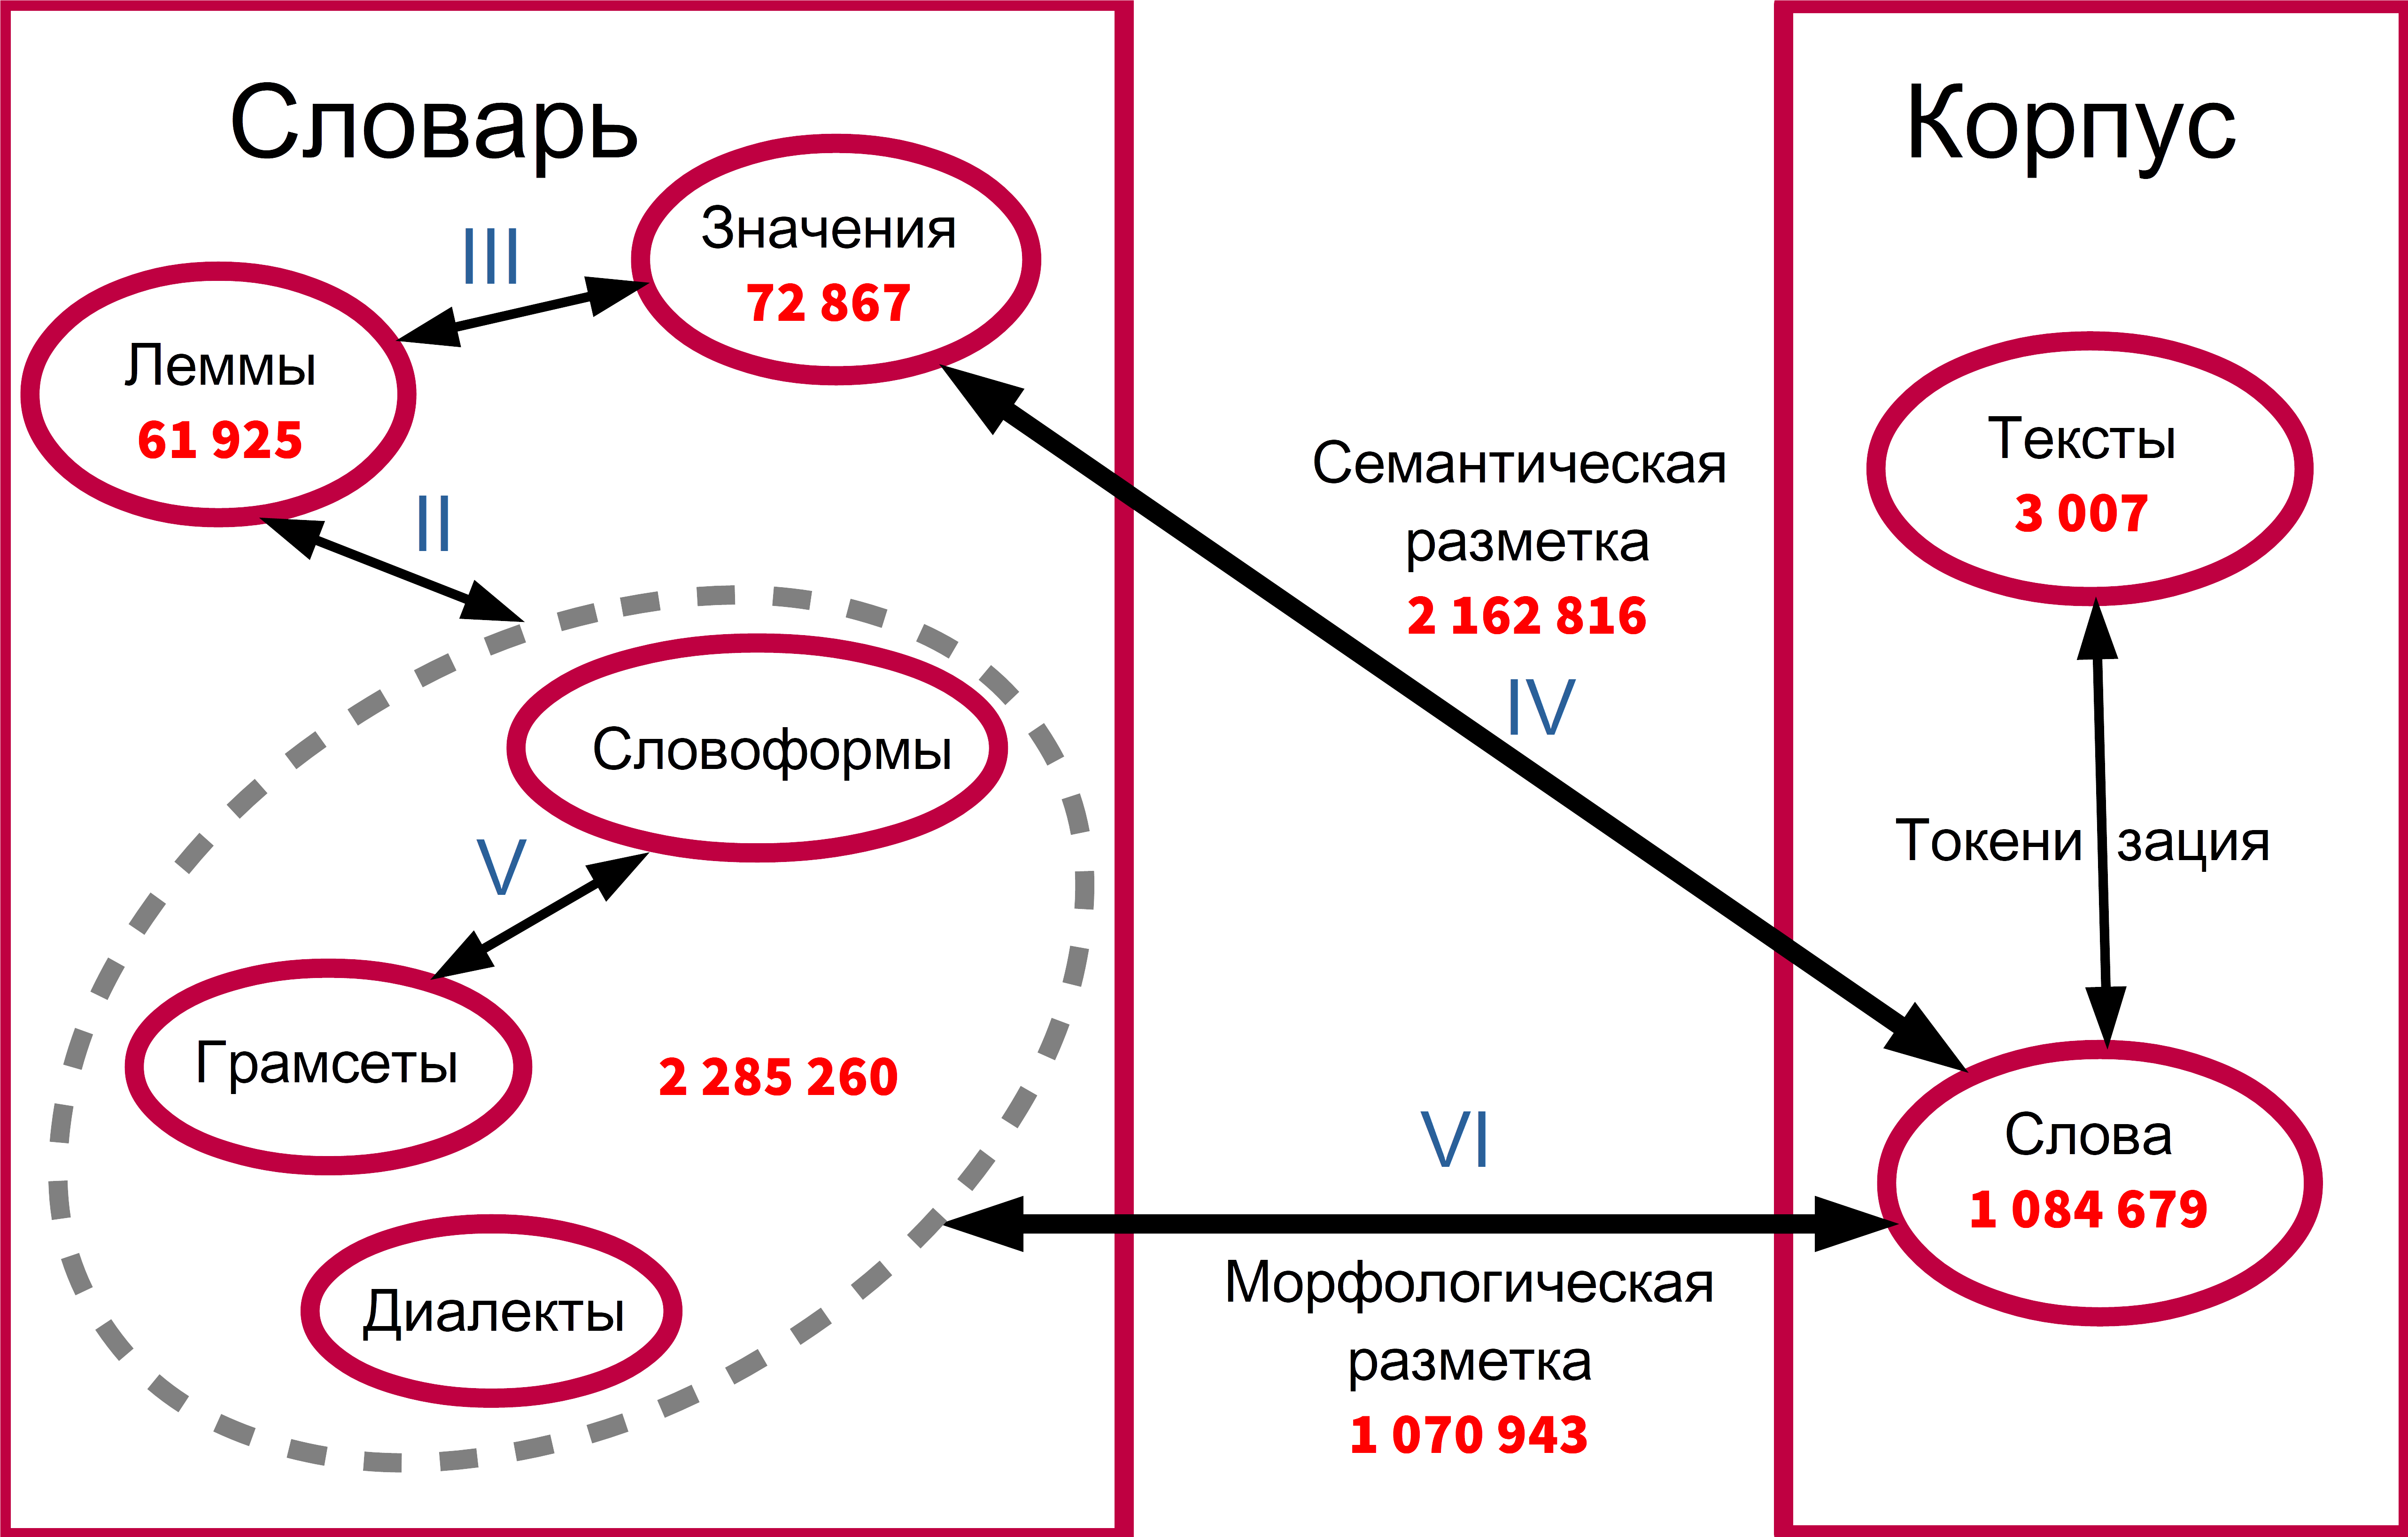
\includegraphics[width=1.0\textwidth,keepaspectratio=true]{corpus_manager_tagging.png}
\caption[Организация данных и разметка текста в корпуса ВепКар]{Организация 
данных и разметка текста в корпуса ВепКар, 
числовые данные приведены по всем языкам и диалектам. Данные на 10 февраля 2021 г.} \label{fig:corpus_manager_tagging}
\end{figure}

Корпусный менеджер обслуживает  словарь и корпус текстов 
(рис.~\ref{fig:corpus_manager_tagging}). 
В текстах выделены границы предложений, в предложениях размечены слова (токены). 
Пример разметки:
\begin{lstlisting}[language=HTML]
<s id="17"><w id="141">Tulow</w> <w id="142">starikku</w> <w id="143">pertih</w>, <w id="144">tuattah</w> <w id="145">se</w>.</s>
\end{lstlisting}

Словарь включает леммы, связанные со значениями, и тройками словоформа--набор грамматических признаков (грамсет\footnote{ \textbf{gramset} -- \textbf{SET} of \textbf{GRAM}matical features})--диалект. 

Система ВепКар при разметке текста автоматически ищет в словаре 
леммы и словоформы, 
совпадающие в написании\footnote{При этом опускаются знаки смягчения (апострофы) 
и заменяются некоторых карельские буквы (в диалектных текстах встречаются буквы, 
которых нет в современном алфавите).
} 
с токенами. 
Это первый этап (\RNum{1}) разметки текста, не представленный на рис.~\ref{fig:corpus_manager_tagging}.  

\begin{enumerate}
\item \textbf{Семантическая разметка}. 
Для найденных в словаре словоформ выбираются связанные с ними леммы (\RNum{2} 
на рис.~\ref{fig:corpus_manager_tagging}), 
потом собираются все значения лемм (\RNum{3}) 
и устанавливаются семантические связи между словами из текста 
и значениями лемм (с пометкой <<не проверено>>) (\RNum{4}). 

%\begin{center}token (word) $\leftrightarrow$ word form $\leftrightarrow$ lemmas $\leftrightarrow$ meanings\end{center}

\begin{tikzpicture}
% TODO mbrace, examples:
% http://www.texample.net/tikz/examples/model-physics/
% http://www.texample.net/tikz/examples/assignment-structure/
% https://ipfs-sec.stackexchange.cloudflare-ipfs.com/tex/A/question/195131.html

%Nodes
\node (token)               {токены (слова)};
\node (wf) [right=of token] {словоформы};
\node (lemma) [right=of wf] {леммы};
\node (meaning) [right=of lemma] {значения};

%Lines
\draw[<->] (token.east) -- node[above] {\RNum{1}} (wf.west);
\draw[<->] (lemma.east) -- node[above] {\RNum{3}} (meaning.west);
\draw[<->] (wf.east) -- node[above] {\RNum{2}} (lemma.west);
\path[<->,red] (token.south) edge [bend right=13] node[above] {этап \RNum{4} не проверен} (meaning.south);
\end{tikzpicture}

%\begin{center}token (word) $\leftrightarrow$ word form $\leftrightarrow$ lemmas $\leftrightarrow$ meanings\end{center}

Задача эксперта-лингвиста~--- проверить эти связи и подтвердить их корректность, 
либо выбрать верную связь из нескольких возможных, 
либо вручную добавить новую словоформу, лемму или значение. 

Когда редактор (эксперт) кликает на токен в тексте, 
появляется выпадающий список всех значений найденных лемм. 
Редактор выбирает правильную лемму и значение (рис.~\ref{fig:text_tagging_by_editor}\footnote{
Полный текст доступен онлайн в корпусе ВепКар. 
См. страницу корпуса с этим текстом \url{http://dictorpus.krc.karelia.ru/en/corpus/text/494}.}). 

% samarialaine: http://dictorpus.krc.karelia.ru/en/corpus/text/494
% 
\begin{figure}
    \centering
    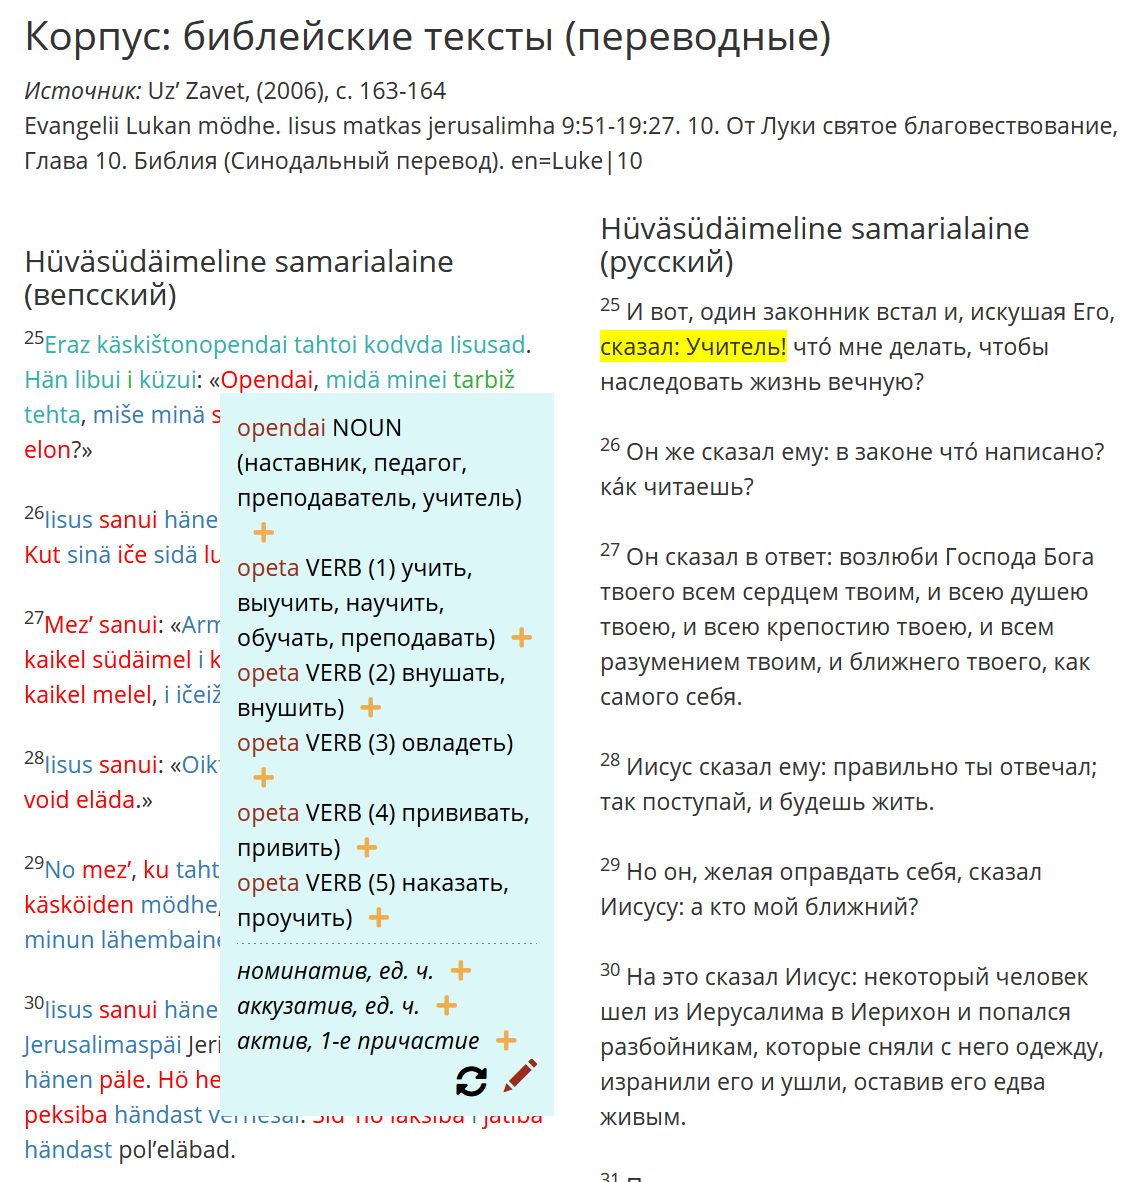
\includegraphics[width=1.0\textwidth,keepaspectratio=true]{text_tagging_by_editor.png}
\caption[Параллельный перевод текстов Библии]{Параллельный перевод текстов Библии: вепсский и русский языки. 
При клике в тексте по слову ``Opendai'' всплывает меню. 
Меню содержит значение для существительного <<учитель>> и пять значений для глагола. 
Когда редактор выбирает одно из значений, кликнув на знак $+$, 
то тем самым связывает токен и значение леммы ({\color{red}этап \RNum{4} проверен}).}
 \label{fig:text_tagging_by_editor}
\end{figure}

\item \textbf{Морфологическая разметка}. 
Для найденных словоформ выбираются связанные с ними грамсеты  (\RNum{5}) и устанавливаются морфологические связи (\RNum{6}) между словами из текста и парами ``словоформа — грамсет'' (Fig.~\ref{fig:text_tagging_by_editor}). 
Задача эксперта -- выбрать правильный грамсет.

\begin{tikzpicture}
%Nodes
\node (token)               {токены (слова)};
\node (wf) [right=of token] {словоформы};
\node (gramset) [right=of wf] {грамсеты};

%Lines
\draw[<->] (token.east) -- node[above] {\RNum{1}} (wf.west);
\draw[<->] (wf.east) -- node[above] {\RNum{5}} (gramset.west);
\path[<->,red] (token.south) edge [bend right=13] node[above] {\RNum{6}} (gramset.south);
\end{tikzpicture}

\end{enumerate}

Как отмечает Т. Архангельский для малоресурсных языков важно, чтобы при автоматическом морфологическом анализе сохранялись в разметке все возможные формы слова для последующей проверки и выбора правильной формы лингвистом~\cite[61]{Arkhangelskiy2020}. Архангельский Т. называет такой корпусный менеджер в корпусе «дружественным к неоднозначности», такой “ambiguity-friendly” платформой является при разметке корпус ВепКар.
%Следующим этапом работы является работа экспертов по проверке разметки и снятию семантической (выбор значения) и морфологический (выбор грамматических признаков) омонимии. 
Например, на рис.~\ref{fig:semantic_and_morph_omonymy} для карельского слова “missä” было найдено три значения местоимения “mi” (что; сколько, что; какой), одно значение наречия “missä” (где) и один набор грамматических признаков (инессив, ед. ч.; наречие - неизменяемое слово, без грамсетов). Для слова “muissa” было найдено одно значения глагола “muistua”, одно значение местоимения “muu” и три грамсета (одно для именной части речи и два для глагола). Эксперт кликая на иконку “плюс” выбирает правильное значение и правильный грамсет.

\begin{figure}
    \centering
    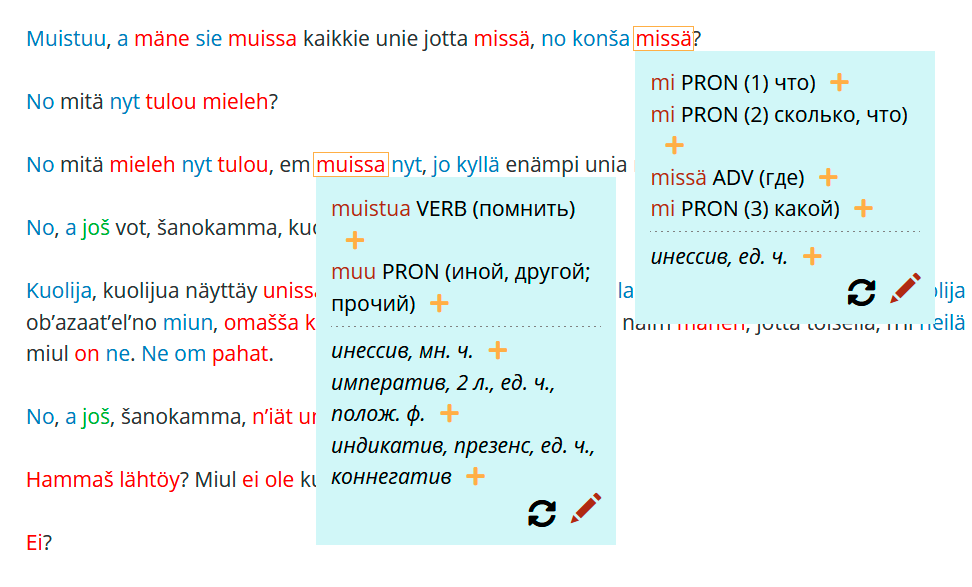
\includegraphics[width=1.0\textwidth,keepaspectratio=true]{vepkar_interface/semantic_and_morph_omonymy.png}
   \caption[Примеры семантической и морфологической омонимии в разметке текста корпуса ВепКар]{Примеры семантической и морфологической омонимии  в разметке текста корпуса ВепКар. 
Для карельского слова “missä” было найдено три значения местоимения “mi”, одно значение наречия “missä” и один грамсет. Для слова “muissa” было найдено одно значения глагола “muistua”, одно значение местоимения “muu” и три грамсета.} 
   \label{fig:semantic_and_morph_omonymy}
\end{figure}
 
\subsubsection{Особенности разметки корпуса ВепКар}\label{corpus_peculiarities}
В этом разделе опишем такую особенность разметки корпуса, из-за которой в описанных выше алгоритмах поиска не учитываются словоформы с пробелами и аналитические формы.
Aнaлитичecкaя фopмa – этo cocтaвнaя фopмa, oбpaзyeмaя coчeтaниeм вспомогательного и полнозначного слова.
Конечной целью настоящей работы является морфологическая разметка текста, предварительно разбитого на слова по пробельным и неалфавитным символам (например: скобки, знаки пунктуации, цифры). 
В имеющихся данных аналитические формы в тексте нам недоступны. 
Хотя в словаре мы храним полные парадигмы, в том числе и аналитические формы, в анализе текста подобные формы не участвуют, поскольку в тексте анализируется каждое отдельное слово, а не группа слов. 

Например, возьмем карельский глагол ‘pageta’ (уйти, убежать).
В словаре мы храним не только отрицательную форму 1 л. ед. ч. презенса индикатива: ‘en pagene’, но и коннегатив индикатива, презенс: ‘pagene’, который участвует в построении пяти из шести форм индикатива, презенс. 
Таким образом, в тексте будет размечено отдельно слово ‘en’ (вспомогательный глагол ‘ei’, индикатив, 1 л., ед. ч.) и отдельно ‘pagene’ (глагол ‘pageta’, коннегатив индикатива, презенс).
 

% Приложения корпуса ВепКар в международных проектах
\subsection{Приложения корпуса ВепКар в международных проектах} \label{sect_VepKar_international}


Отметим важность и востребованность работ по развитию корпуса текстов. 
Во-первых, в соревновании <<Оценка методов обработки малоресурсных языков>>, 
проведённом в феврале-марте 2019 года 
в рамках международной конференции <<Диалог>>, 
использовались размеченные данные корпуса ВепКар 
в формате CONLL~\cite{Klyachko2019LowresourceEval}. 
Результаты соревнования и данные корпусов 
доступны онлайн\footnote{См. \url{https://lowresource-lang-eval.github.io}}.

Во-вторых, данные корпуса с 2019 года включены 
в международную морфологическую базу данных 
UniMorph\footnote{См. \url{https://github.com/unimorph}}~\cite{McCarthy2020Unimorph}. 
Экспорт данных в общепринятые форматы (CONLL, UniMorph) 
важен для привлечения к исследованию вепсского и карельского языков 
международного научного сообщества. 
В последние годы становится практикой, 
когда новые методы и алгоритмы вычислительной лингвистики 
проверяются не на одном-двух языках, 
а на множестве языков, например, с привлечением базы UniMorph, включающей 110 языков. 
Таким образом, теперь в эту сотню языков входят вепсский язык и три диалекта карельского языка. 
\TODO{TODO: привести фрагмент таблицы с результатами вычислений по этим языкам (выборка из большой таблицы, см. Overleaf)}.

Новые данные вепсского и карельских словарей корпуса ВепКар экспортированы и включены в международный проект UniMorph 3.0 (международная морфологическая разметка):
* вепсский язык (https://github.com/unimorph/vep),
* собственно карельское наречие (https://github.com/unimorph/krl),
* карельский: ливвиковское наречие (https://github.com/unimorph/olo),
* карельский: людиковское наречие (https://github.com/unimorph/lud).

Был разработан специальный модуль для экспорта текстов в формате CONLL и 
для экспорта словарей в формате UD для проекта UniMorph \aka{Ссылки на статью и проект ~Tree Dependency Bank по ВепКар}.
  











